\documentclass[11pt,a4paper,openany]{book}

\usepackage[utf8]{inputenc}
\usepackage[T1]{fontenc}
\usepackage{amsmath,amssymb,amsfonts,amsthm}
\usepackage{geometry}
\geometry{a4paper, left=2.2cm, right=2.2cm, top=2.5cm, bottom=2.5cm}

\usepackage{booktabs}
\usepackage{array}
\usepackage{longtable}
\usepackage{pdfpages}
\usepackage{csquotes}
\MakeOuterQuote{"}

\usepackage{xcolor}
\definecolor{mosaicblue}{RGB}{74, 128, 196}
\definecolor{mosaicpink}{RGB}{224, 102, 102}

\usepackage{tikz}
\usetikzlibrary{shapes.geometric, calc}

\usepackage[pdfusetitle, hidelinks, colorlinks=true, linkcolor=blue!70!black, citecolor=blue!70!black, urlcolor=blue!70!black]{hyperref}

\title{\textbf{The Polygonal Burnsidean}\\[0.4em]
\Large An Atlas of Inscribed Polygons from $\mathbb{Z}_1$ to $\mathbb{Z}_{16}$}
\author{Gemma Knee \and Antigra Vitti}
\date{November 2026}

\begin{document}

\frontmatter
\maketitle

\chapter*{Preface}
\addcontentsline{toc}{chapter}{Preface}
\markboth{Preface}{Preface}

This volume presents a complete catalogue and algebraic
classification of single inscribed polygons on circular lattice
rings from the singleton $\mathbb{Z}_1$ to the hexadecagonal ring
$\mathbb{Z}_{16}$.

While general composition mosaics exhibit factorial combinatorial
growth governed by the Bell numbers—yielding billions of multi-block
partitions on higher-order lattices—the geometry of a single inscribed
polygon corresponds to the fundamental Cauchy--Frobenius cycle index substitution
$z_k \mapsto 1 + x^k$. Across the circular rings from $\mathbb{Z}_1$
to $\mathbb{Z}_{16}$, this universe encompasses the complete catalogue
of non-equivalent dihedral configurations under the physical symmetries
of $D_n$.

In this comprehensive edition, we establish the foundational cartography of these single-polygon shapes:
\begin{itemize}
    \item Every orbit is depicted in a canonical geometric orientation, within an ambient regular polygon frame with inscribed vertices, metric chords, and shaded polygonal tiles.
    \item Two-colour chromatic coding distinguishes bilaterally symmetric configurations (blue) from scalene, chiral enantiomorphs (pink).
    \item The companion machine-readable dataset provides the canonical circular composition sequence for every orbit, detailing the circular strides connecting adjacent lattice vertices.
\end{itemize}

\bigskip
\begin{flushright}
\textbf{Gemma Knee} \qquad \textbf{Antigra Vitti} \\
\emph{Newcastle upon Tyne} \\
\emph{November 2026}
\end{flushright}


\tableofcontents

\mainmatter

\chapter{Lattice Geometry and Inscribed Polygons}
\label{chap:polygon-geometry}

\section{The Inscribed Polygon Universe}

Let $\mathbb{Z}_n = \{0, 1, \dots, n-1\}$ denote the cyclic ring of
integers modulo $n$, drawn as the vertices of a regular
$n$-gon in the Euclidean plane, oriented with vertex $0$ at the top
and indices advancing clockwise. The physical symmetries of this circular
lattice constitute the dihedral group $D_n$ of order $2n$, generated by
the unit rotation $\rho \colon x \mapsto x + 1 \pmod n$ and the vertical
bilateral reflection $\tau \colon x \mapsto -x \equiv n - x \pmod n$.

An \textbf{inscribed polygon} in $\mathbb{Z}_n$ is specified by an
arbitrary subset of vertices $S \subseteq \mathbb{Z}_n$ of cardinality
$k = |S| \in \{0, 1, \dots, n\}$:
\begin{itemize}
    \item For $k = 0$, $S = \emptyset$ represents the empty polygon.
    \item For $k = 1$, $S = \{v\}$ represents a unigon (isolated vertex).
    \item For $k = 2$, $S = \{u, v\}$ represents a digon (a line of circular span $\min(|u-v|, n-|u-v|)$).
    \item For $3 \le k \le n-1$, $S$ represents a convex $k$-gon inscribed within the lattice.
    \item For $k = n$, $S = \mathbb{Z}_n$ spans the complete $n$-gon.
\end{itemize}

\noindent\textbf{Degenerate Base Lattices: $\mathbb{Z}_1$ and $\mathbb{Z}_2$}\\[0.5em]

The degenerate base rings $\mathbb{Z}_1$ and $\mathbb{Z}_2$ admit trivial
dihedral symmetry groups ($D_1 \cong C_2$ and $D_2 \cong C_2 \times
C_2$). While excluded from the main catalogue plates, their complete
subset universes are fully enumerated:

\begin{figure}[htbp]
\centering
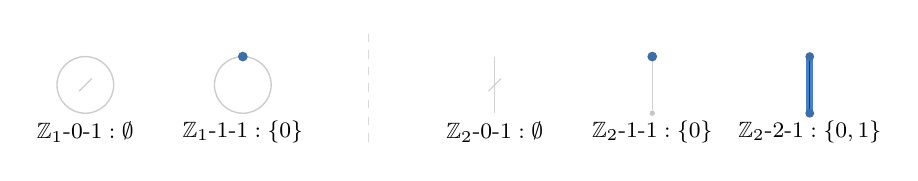
\begin{tikzpicture}[scale=0.8, baseline=-0.5ex]
    % Z_1: empty
    \begin{scope}[shift={(0,0)}]
        \draw[gray!40, line width=0.5pt] (0,0) circle (0.45cm);
        \draw[gray!40, line width=0.4pt] (-0.1,-0.1) -- (0.1,0.1);
        \node[font=\footnotesize\sffamily] at (0,-0.75) {$\mathbb{Z}_1\text{-}0\text{-}1: \emptyset$};
    \end{scope}
    % Z_1: unigon
    \begin{scope}[shift={(2.5,0)}]
        \draw[gray!40, line width=0.5pt] (0,0) circle (0.45cm);
        \fill[mosaicblue!85!black] (0,0.45) circle (2.2pt);
        \node[font=\footnotesize\sffamily] at (0,-0.75) {$\mathbb{Z}_1\text{-}1\text{-}1: \{0\}$};
    \end{scope}
    % Divider
    \draw[gray!30, dashed] (4.5,-0.9) -- (4.5,0.9);
    % Z_2: empty
    \begin{scope}[shift={(6.5,0)}]
        \draw[gray!35, line width=0.5pt] (0,0.45) -- (0,-0.45);
        \draw[gray!40, line width=0.4pt] (-0.1,-0.1) -- (0.1,0.1);
        \node[font=\footnotesize\sffamily] at (0,-0.75) {$\mathbb{Z}_2\text{-}0\text{-}1: \emptyset$};
    \end{scope}
    % Z_2: unigon
    \begin{scope}[shift={(9.0,0)}]
        \draw[gray!35, line width=0.5pt] (0,0.45) -- (0,-0.45);
        \fill[mosaicblue!85!black] (0,0.45) circle (2.2pt);
        \fill[gray!45] (0,-0.45) circle (1.2pt);
        \node[font=\footnotesize\sffamily] at (0,-0.75) {$\mathbb{Z}_2\text{-}1\text{-}1: \{0\}$};
    \end{scope}
    % Z_2: digon
    \begin{scope}[shift={(11.5,0)}]
        \draw[mosaicblue, line width=2.4pt, line cap=round] (0,0.45) -- (0,-0.45);
        \draw[black!80, line width=0.4pt, line cap=round] (0,0.45) -- (0,-0.45);
        \fill[mosaicblue!85!black] (0,0.45) circle (2.0pt);
        \fill[mosaicblue!85!black] (0,-0.45) circle (2.0pt);
        \node[font=\footnotesize\sffamily] at (0,-0.75) {$\mathbb{Z}_2\text{-}2\text{-}1: \{0,1\}$};
    \end{scope}
\end{tikzpicture}
\caption{\label{fig:degenerate-rings}All Inscribed Subsets of $\mathbb{Z}_1$ (2 Orbits) and $\mathbb{Z}_2$ (3 Orbits)}
\end{figure}

\section{The Cauchy--Frobenius Polynomial \texorpdfstring{$CF_n(x)$}{CFn(x)}}

In combinatorial enumeration under group action, the total number of
non-equivalent $k$-element subsets under the dihedral group $D_n$ is
governed by the Cauchy--Frobenius lemma (often historically misattributed
to Burnside) applied via P\'olya's cycle index $Z(D_n; z_1, z_2, \dots, z_n)$.

Evaluating the cycle index under the binary substitution $z_k \mapsto
1 + x^k$ produces the \emph{Cauchy--Frobenius bracelet generating polynomial}:

\begin{equation}
CF_n(x) = Z\left(D_n; 1 + x, 1 + x^2, \dots, 1 + x^n\right) = \sum_{k=0}^n c_{n,k} x^k
\end{equation}
where $c_{n,k}$ is the exact number of dihedral orbits of inscribed $k$-gons.

For odd $n = 2m + 1$, every reflection possesses one fixed vertex and $m$ chords:
\begin{equation}
Z(D_n) = \frac{1}{2n} \left( \sum_{d \mid n} \phi(d) z_d^{n/d} + n z_1 z_2^{(n-1)/2} \right)
\end{equation}
For even $n = 2m$, the $n$ reflections decompose into $n/2$ vertex-vertex axes and $n/2$ edge-edge axes:
\begin{equation}
Z(D_n) = \frac{1}{2n} \left( \sum_{d \mid n} \phi(d) z_d^{n/d} + \frac{n}{2} z_1^2 z_2^{(n-2)/2} + \frac{n}{2} z_2^{n/2} \right)
\end{equation}

Evaluating $CF_n(1)$ by setting $x = 1$ yields the total number of dihedral subset orbits on $\mathbb{Z}_n$.

\section{Complement Duality and Bilateral Symmetry}

Two geometric dualities govern the atlas:

\begin{enumerate}
    \item \textbf{Complement Duality ($k \longleftrightarrow n - k$)}:
    The mapping $S \mapsto \mathbb{Z}_n \setminus S$ defines an isometric bijection between $k$-gons and $(n-k)$-gons. Because the cycle index polynomial is palindromic:
    \begin{equation}
    c_{n,k} \equiv c_{n, n-k}
    \end{equation}
    Every $k$-gon has a canonical complementary $(n-k)$-gon. When $n$ is even, polygons at the central equator $k = n/2$ can be \emph{self-complementary} under dihedral symmetry.
    
    \item \textbf{Bilateral Reflection Symmetry (Chirality)}:
    An inscribed polygon $S$ is \textbf{achiral} (shaded in blue) if there exists a reflection $\tau \in D_n$ such that $\tau(S) = S$. Absent such reflection, $S$ is \textbf{chiral} (shaded in pink), existing as one member of an enantiomorphic pair $(S, \tau(S))$ that split into distinct orbits under cyclic rotations $C_n$.
\end{enumerate}

\chapter{The Dihedral Polygon Census}
\label{chap:harmonic-taxonomy}

\section{Census from \texorpdfstring{$\mathbb{Z}_1$ to $\mathbb{Z}_{16}$}{Z1 to Z16}}

Table~\ref{tab:poly-census-summary} details the complete census of
non-equivalent dihedral and cyclic inscribed polygon orbits across the
circular rings $\mathbb{Z}_1$ through $\mathbb{Z}_{16}$.

% Summary Table of Inscribed Polygon Orbits Z_1 to Z_16
\begin{table}[htbp]
\centering\small
\caption{\label{tab:poly-census-summary}Dihedral Polygon Orbit Census from $\mathbb{Z}_1$ to $\mathbb{Z}_{16}$}
\begin{tabular}{r | r r | r r | r r}
\toprule
Ring $\mathbb{Z}_n$ & $2^n$ Subsets & $|D_n|$ & Dihedral Orbits & Cyclic Orbits & Chiral Pairs & Chiral \% \\
\midrule
$\mathbb{Z}_{1}$ & 2 & 2 & \textbf{2} & 2 & 0 & 0.0\% \\
$\mathbb{Z}_{2}$ & 4 & 4 & \textbf{3} & 3 & 0 & 0.0\% \\
$\mathbb{Z}_{3}$ & 8 & 6 & \textbf{4} & 4 & 0 & 0.0\% \\
$\mathbb{Z}_{4}$ & 16 & 8 & \textbf{6} & 6 & 0 & 0.0\% \\
$\mathbb{Z}_{5}$ & 32 & 10 & \textbf{8} & 8 & 0 & 0.0\% \\
$\mathbb{Z}_{6}$ & 64 & 12 & \textbf{13} & 14 & 1 & 7.7\% \\
$\mathbb{Z}_{7}$ & 128 & 14 & \textbf{18} & 20 & 2 & 11.1\% \\
$\mathbb{Z}_{8}$ & 256 & 16 & \textbf{30} & 36 & 6 & 20.0\% \\
$\mathbb{Z}_{9}$ & 512 & 18 & \textbf{46} & 60 & 14 & 30.4\% \\
$\mathbb{Z}_{10}$ & 1,024 & 20 & \textbf{78} & 108 & 30 & 38.5\% \\
$\mathbb{Z}_{11}$ & 2,048 & 22 & \textbf{126} & 188 & 62 & 49.2\% \\
$\mathbb{Z}_{12}$ & 4,096 & 24 & \textbf{224} & 352 & 128 & 57.1\% \\
$\mathbb{Z}_{13}$ & 8,192 & 26 & \textbf{380} & 632 & 252 & 66.3\% \\
$\mathbb{Z}_{14}$ & 16,384 & 28 & \textbf{687} & 1,182 & 495 & 72.1\% \\
$\mathbb{Z}_{15}$ & 32,768 & 30 & \textbf{1224} & 2,192 & 968 & 79.1\% \\
$\mathbb{Z}_{16}$ & 65,536 & 32 & \textbf{2250} & 4,116 & 1,866 & 82.9\% \\
\bottomrule
\end{tabular}
\end{table}


The census reveals a phase transition in the emergence of chiral asymmetry:
\begin{itemize}
    \item On small rings $\mathbb{Z}_1$ through $\mathbb{Z}_5$, every
    inscribed polygon is strictly bilaterally symmetric ($0\%$ chirality).
    \item Chirality first emerges on $\mathbb{Z}_6$ at size $k=3$:
    the unique scalene triangle $\texttt{/013/}$, whose reflection
    $\texttt{/023/}$ forms an enantiomorphic partner.
    \item Chirality expands steadily through $\mathbb{Z}_8$ ($20.0\%$),
    crosses the $50\%$ majority mark at $\mathbb{Z}_{12}$ ($57.1\%$),
    and reaches $82.9\%$ at $\mathbb{Z}_{16}$, where $1{,}866$ of the
    $2{,}250$ orbits are chiral enantiomorphs.
\end{itemize}

\section{Analytical Invariants and Digital Resource}

Each orbit is uniquely identified by its canonical circular stride
composition word $c_1 \dots c_k$ (with digit sum $n$ and length
$k$), local atlas designation $k\text{-}i$, canonical vertex subset
representative in hexadecimal slash notation $/v_1 \dots v_k/$, dihedral
orbit length $|\mathcal{O}|$, and binary bilateral reflection flag ($1 =
\text{achiral}$, $0 = \text{chiral}$).

The complete 5{,}099-orbit inventory is maintained in the companion
files \path{data/inngons.tsv}, \path{inngons.csv}, and \path{inngons.json}
for computational querying and stream filtering.

\chapter{The Visual Atlas of Inscribed Polygons}
\label{chap:visual-atlas}

\section*{Cartographic Conventions}

This catalogue displays the complete census of non-equivalent
dihedral inscribed polygons across the circular rings $\mathbb{Z}_1$
through $\mathbb{Z}_{16}$, organized sequentially ring by ring.

Each drawing portrays an individual dihedral orbit in its canonical orientation:
\begin{itemize}
    \item \textbf{Lattice Geometry}: The ambient circular lattice $\mathbb{Z}_n$ is the regular $n$-gon with vertex $0$ positioned at the top and indices advancing clockwise $0, 1, \dots, n-1$. Faint pips mark unselected vertices.
    \item \textbf{Polygonal Hierarchy}:
    \begin{itemize}
        \item \emph{Empty Polygons ($k=0$)} are marked by an ambient wireframe with a central null indicator.
        \item \emph{Unigons ($k=1$)} are marked by a prominent circular node at the active vertex.
        \item \emph{Digons ($k=2$)} are drawn as bold lines connecting the vertex pair.
        \item \emph{Polygons ($k \ge 3$)} are drawn as shaded polygonal tiles bounded by perimeter chords and solid vertex nodes.
    \end{itemize}
    \item \textbf{Bilateral Symmetry Colouring}:
    \begin{itemize}
        \item \textbf{Blue}: Bilaterally symmetric (achiral) polygons have (at least) one internal axis of dihedral reflection.
        \item \textbf{Pink}: Scalene (chiral) polygons lack reflection symmetry.
    \end{itemize}
    \item \textbf{Coordinate Annotations}:
    \begin{itemize}
        \item \textbf{Upper-Left Designation}: Bold cardinality-and-rank index ($k\text{-}i$) indicates the $i$-th non-equivalent $k$-gon on the active lattice ring, cross-referenced with the analytical dataset.
        \item \textbf{Lower-Right Orbit Size}: Dihedral orbit length $|\mathcal{O}| \in \{1, 2, \dots, 2n\}$ under the action of $D_n$.
    \end{itemize}
\end{itemize}

\bigskip
\noindent\textit{Degenerate Base Lattices}: The unigonal and digonal configurations on the degenerate rings $\mathbb{Z}_1$ and $\mathbb{Z}_2$ are illustrated in Figure~\ref{fig:degenerate-rings} of Chapter~\ref{chap:polygon-geometry}. The visual atlas plates begin with the triangular ring $\mathbb{Z}_3$ on Plate~1.

\clearpage
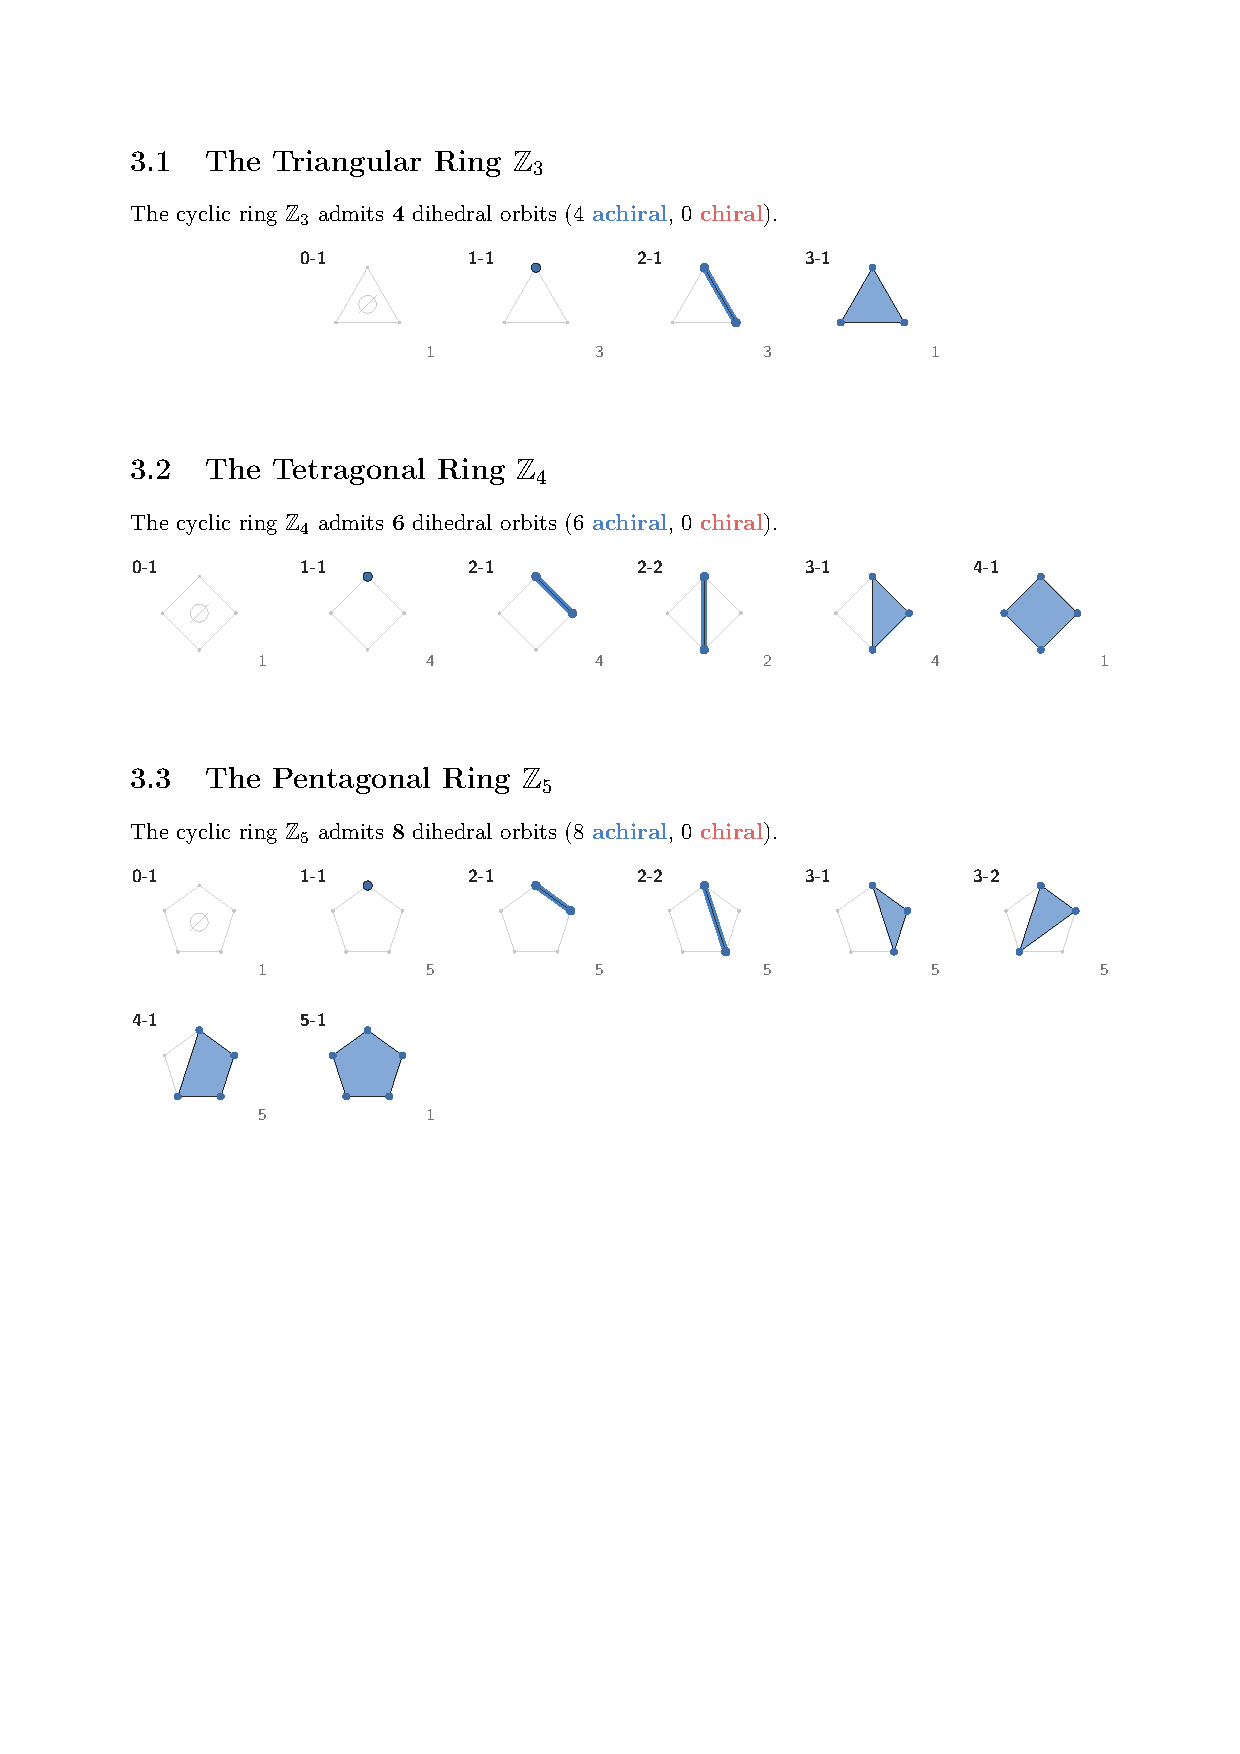
\includepdf[
  pages=-,
  pagecommand={\thispagestyle{headings}},
  addtotoc={
     1, section, 1, {The Triangular Ring \texorpdfstring{$\mathbb{Z}_3$}{Z3}}, sec:ring-z3,
     1, section, 1, {The Tetragonal Ring \texorpdfstring{$\mathbb{Z}_4$}{Z4}}, sec:ring-z4,
     1, section, 1, {The Pentagonal Ring \texorpdfstring{$\mathbb{Z}_5$}{Z5}}, sec:ring-z5,
     2, section, 1, {The Hexagonal Ring \texorpdfstring{$\mathbb{Z}_6$}{Z6}}, sec:ring-z6,
     2, section, 1, {The Heptagonal Ring \texorpdfstring{$\mathbb{Z}_7$}{Z7}}, sec:ring-z7,
     3, section, 1, {The Octagonal Ring \texorpdfstring{$\mathbb{Z}_8$}{Z8}}, sec:ring-z8,
     4, section, 1, {The Enneagonal Ring \texorpdfstring{$\mathbb{Z}_9$}{Z9}}, sec:ring-z9,
     5, section, 1, {The Decagonal Ring \texorpdfstring{$\mathbb{Z}_{10}$}{Z10}}, sec:ring-z10,
     7, section, 1, {The Hendecagonal Ring \texorpdfstring{$\mathbb{Z}_{11}$}{Z11}}, sec:ring-z11,
    10, section, 1, {The Dodecagonal Ring \texorpdfstring{$\mathbb{Z}_{12}$}{Z12}}, sec:ring-z12,
    15, section, 1, {The Tridecagonal Ring \texorpdfstring{$\mathbb{Z}_{13}$}{Z13}}, sec:ring-z13,
    23, section, 1, {The Tetradecagonal Ring \texorpdfstring{$\mathbb{Z}_{14}$}{Z14}}, sec:ring-z14,
    36, section, 1, {The Pentadecagonal Ring \texorpdfstring{$\mathbb{Z}_{15}$}{Z15}}, sec:ring-z15,
    59, section, 1, {The Hexadecagonal Ring \texorpdfstring{$\mathbb{Z}_{16}$}{Z16}}, sec:ring-z16
  }
]{plates/poly_plates.pdf}


\backmatter
\chapter*{Suggested Reading}
\addcontentsline{toc}{chapter}{Suggested Reading}
\markboth{Suggested Reading}{Suggested Reading}

This atlas bridges the geometry of inscribed convex polygons with permutation group actions and circular composition combinatorics. The curated works below provide foundational theory, classical historical developments, and broader algebraic context.

\section*{Dihedral Enumeration and Group Actions}

\begin{description}
    \item[\textbf{Augustin-Louis Cauchy (1845)}]\mbox{}\\
    \emph{M\'emoire sur diverses propri\'et\'es remarquables des substitutions r\'eguli\`eres ou irr\'eguli\`eres, et des syst\`emes de substitutions conjugu\'ees}, \emph{Comptes Rendus de l'Acad\'emie des Sciences}, 21:972--987.\\
    The original formulation of the orbit-counting lemma for permutation groups.

    \item[\textbf{Ferdinand Georg Frobenius (1887)}]\mbox{}\\
    \emph{\"Uber die Congruenz nach einem aus zwei endlichen Gruppen gebildeten Doppelmodul}, \emph{Journal f\"ur die reine und angewandte Mathematik (Crelle's Journal)}, 101:273--299.\\
    The generalisation of the orbit-counting theorem to abstract finite group actions.

    \item[\textbf{William Burnside (1911)}]\mbox{}\\
    \emph{Theory of Groups of Finite Order}, 2nd edition, Cambridge University Press, Cambridge.\\
    The classical treatise popularising the orbit-counting lemma (attributing the theorem to Frobenius in Section~118), forming the arithmetic core of dihedral cycle index evaluations.

    \item[\textbf{Peter M. Neumann (1979)}]\mbox{}\\
    \emph{A story that is not Burnside's}, \emph{The Mathematical Gazette}, 63(426):271--270.\\
    A delightful historical account detailing the provenance of the Cauchy--Frobenius lemma and its popular misattribution to Burnside.

    \item[\textbf{J. Howard Redfield (1927)}]\mbox{}\\
    \emph{The theory of group-reduced distributions}, \emph{American Journal of Mathematics}, 49(3):433--455.\\
    The pioneering paper anticipating P\'olya's enumeration theorems, introducing group-reduced distributions and the superposition of permutation representations.

    \item[\textbf{George P\'olya (1937)}]\mbox{}\\
    \emph{Kombinatorische Anzahlbestimmungen f\"ur Gruppen, Graphen und chemische Verbindungen}, \emph{Acta Mathematica}, 68(1):145--254.\\
    The foundational memoir formalising the cycle index polynomial $Z(G; z_1, \dots, z_n)$ and its functional substitution principles for weighted configuration counting under group equivalence.

    \item[\textbf{Adalbert Kerber (1999)}]\mbox{}\\
    \emph{Applied Finite Group Actions}, 2nd edition, Springer-Verlag, Berlin, Heidelberg.\\
    An exhaustive modern reference on the algebraic and algorithmic apparatus of permutation representations, double-coset decompositions, and constructive orbit generation.
\end{description}

\section*{Cyclic Polygons and Circular Compositions}

\begin{description}
    \item[\textbf{Duncan M. Y. Sommerville (1909)}]\mbox{}\\
    \emph{On Certain Periodic Properties of Cyclic Compositions of Numbers}, \emph{Proceedings of the London Mathematical Society}, Second Series, 7:263--313.\\
    A fundamental early 20th-century investigation into the period structures and symmetry classes of cyclic integer compositions, establishing the combinatorial basis for circular stride sequences.

    \item[\textbf{Hansraj Gupta (1979)}]\mbox{}\\
    \emph{Enumeration of Incongruent Cyclic $k$-gons}, \emph{Indian Journal of Pure and Applied Mathematics}, 10(8):964--999.\\
    An exact combinatorial classification of incongruent convex polygons inscribed in circular lattices under physical rotation and reflection.

    \item[\textbf{E. N. Gilbert and John Riordan (1961)}]\mbox{}\\
    \emph{Symmetry Types of Periodic Sequences}, \emph{Illinois Journal of Mathematics}, 5(4):657--665.\\
    The definitive classification of periodic circular sequences (necklaces and bracelets) under cyclic and dihedral group actions.

    \item[\textbf{Petros Hadjicostas (2017)}]\mbox{}\\
    \emph{Cyclic, Dihedral and Symmetrical Carlitz Compositions of a Positive Integer}, \emph{Journal of Integer Sequences}, 20(8):Article 17.8.5.\\
    A modern treatment of cyclic and dihedral composition spaces with restricted adjacent summands and bilateral symmetry constraints.
\end{description}

\section*{Combinatorial and Graphical Enumeration}

\begin{description}
    \item[\textbf{Richard P. Stanley (2011)}]\mbox{}\\
    \emph{Enumerative Combinatorics}, Volume 1, 2nd edition, Cambridge University Press, Cambridge.\\
    The standard modern reference on generating functions, posets, and group actions on finite sets, including necklace and bracelet algebra.

    \item[\textbf{Frank Harary and Edgar M. Palmer (1973)}]\mbox{}\\
    \emph{Graphical Enumeration}, Academic Press, New York.\\
    A classic, pedagogical text applying P\'olya enumeration techniques to geometric graphs, simplicial complexes, and spatial symmetry classes.

    \item[\textbf{George E. Andrews (1976)}]\mbox{}\\
    \emph{The Theory of Partitions}, Addison-Wesley, Reading, MA.\\
    The authoritative treatise on integer partitions, modular identities, and their geometric realizations.
\end{description}

\section*{Geometric Metric Spaces and Musical Orbifolds}

\begin{description}
    \item[\textbf{Godfried T. Toussaint (2013)}]\mbox{}\\
    \emph{The Geometry of Musical Rhythm: What Makes a ``Good'' Rhythm Good?}, CRC Press, Boca Raton, FL.\\
    A comprehensive geometric investigation into cyclic rhythmic timelines, analysing maximal evenness, convex hulls, and Afro-Cuban clave patterns as inscribed polygons in $\mathbb{Z}_{16}$.

    \item[\textbf{Dmitri Tymoczko (2011)}]\mbox{}\\
    \emph{A Geometry of Music: Harmony and Counterpoint in the Extended Common Practice}, Oxford University Press, New York.\\
    Foundational formulation of musical scales, pitch-class sets, and voice leading as geometric configurations and paths within quotient orbifolds under dihedral and symmetric group actions.
\end{description}


\end{document}
